%%%%%%%%%%%%%%%%%%%%%%%%%%%%%%%%%%%%%%%%%%%%%%%%%%%%%%%%%%%%%%%%%%%%
%% I, the copyright holder of this work, release this work into the
%% public domain. This applies worldwide. In some countries this may
%% not be legally possible; if so: I grant anyone the right to use
%% this work for any purpose, without any conditions, unless such
%% conditions are required by law.
%%%%%%%%%%%%%%%%%%%%%%%%%%%%%%%%%%%%%%%%%%%%%%%%%%%%%%%%%%%%%%%%%%%%

% This theme was based on fibeamer theme 
% If you found any bugs please contact @karlosos
% This repository is hosted on github https://github.com/karlosos/zut-fibeamer/

\documentclass[t]{beamer}
\usetheme[faculty=wi]{fibeamer}
\usepackage[utf8]{inputenc}
\usepackage[
  main=portuguese,
  english
]{babel}

\title{Impacto das modulações do {IEEE 802.15.4g} na qualidade de comunicação em ambiente de \textit{Smart Building}}
\subtitle{Discente: Felipe Ferreira Bezerra da Silva}
\author{Orientador: Prof. Ruan Delgado Gomes, D.Sc.}

\usepackage{ragged2e}  % `\justifying` text
\usepackage{booktabs}  % Tables
\usepackage{tabularx}
\usepackage{tikz}      % Diagrams
\usetikzlibrary{calc, shapes, backgrounds}
\usepackage{amsmath, amssymb}
\usepackage{url}       % `\url`s
\usepackage{listings}  % Code listings
\usepackage{graphicx}
\frenchspacing
\begin{document}
\frame[c]{\maketitle}

\AtBeginSection[]{% Print an outline at the beginning of sections
  \begin{frame}<beamer>
    \frametitle{Seção \thesection}
    \tableofcontents[currentsection]
  \end{frame}}

\begin{darkframes}

  \section{Introdução}
  \begin{frame}{Introdução}
    \framesubtitle{IoT}
    \begin{figure}[ht]
      \centering
      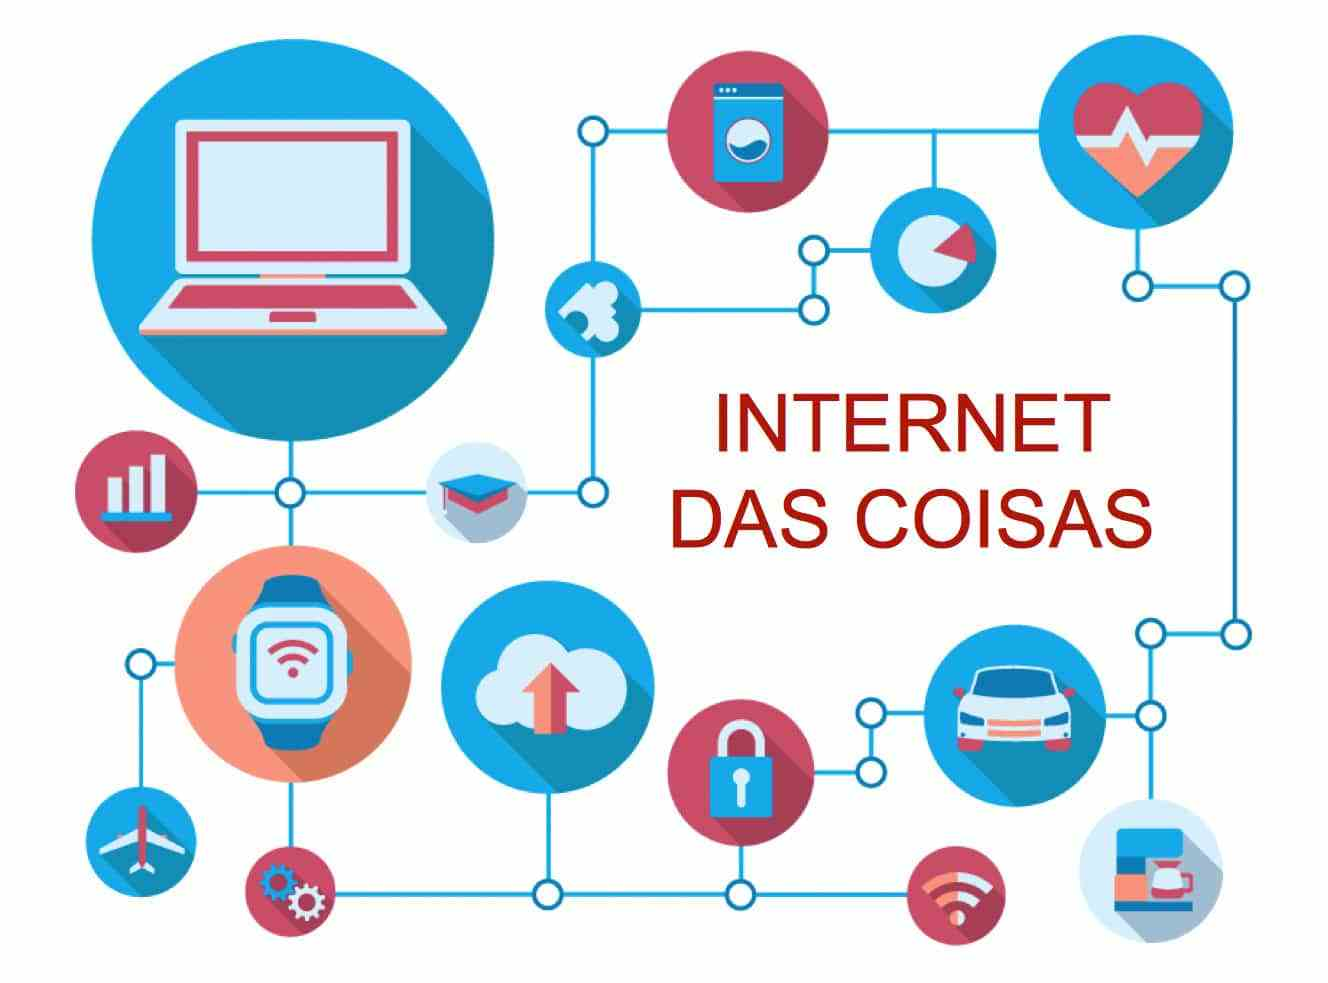
\includegraphics[width=.7\textwidth]{resources/intro_iot.jpg}\\
      \footnotesize{Retirado do site http://sentrybrasil.com.br/cursos/internet-das-coisas-vai-revolucionar-o-mercado/}
    \end{figure}
  \end{frame}

  \begin{frame}{Introdução}
    \framesubtitle{Aplicação - Smart Campus}
    \begin{figure}[ht]
      \centering
      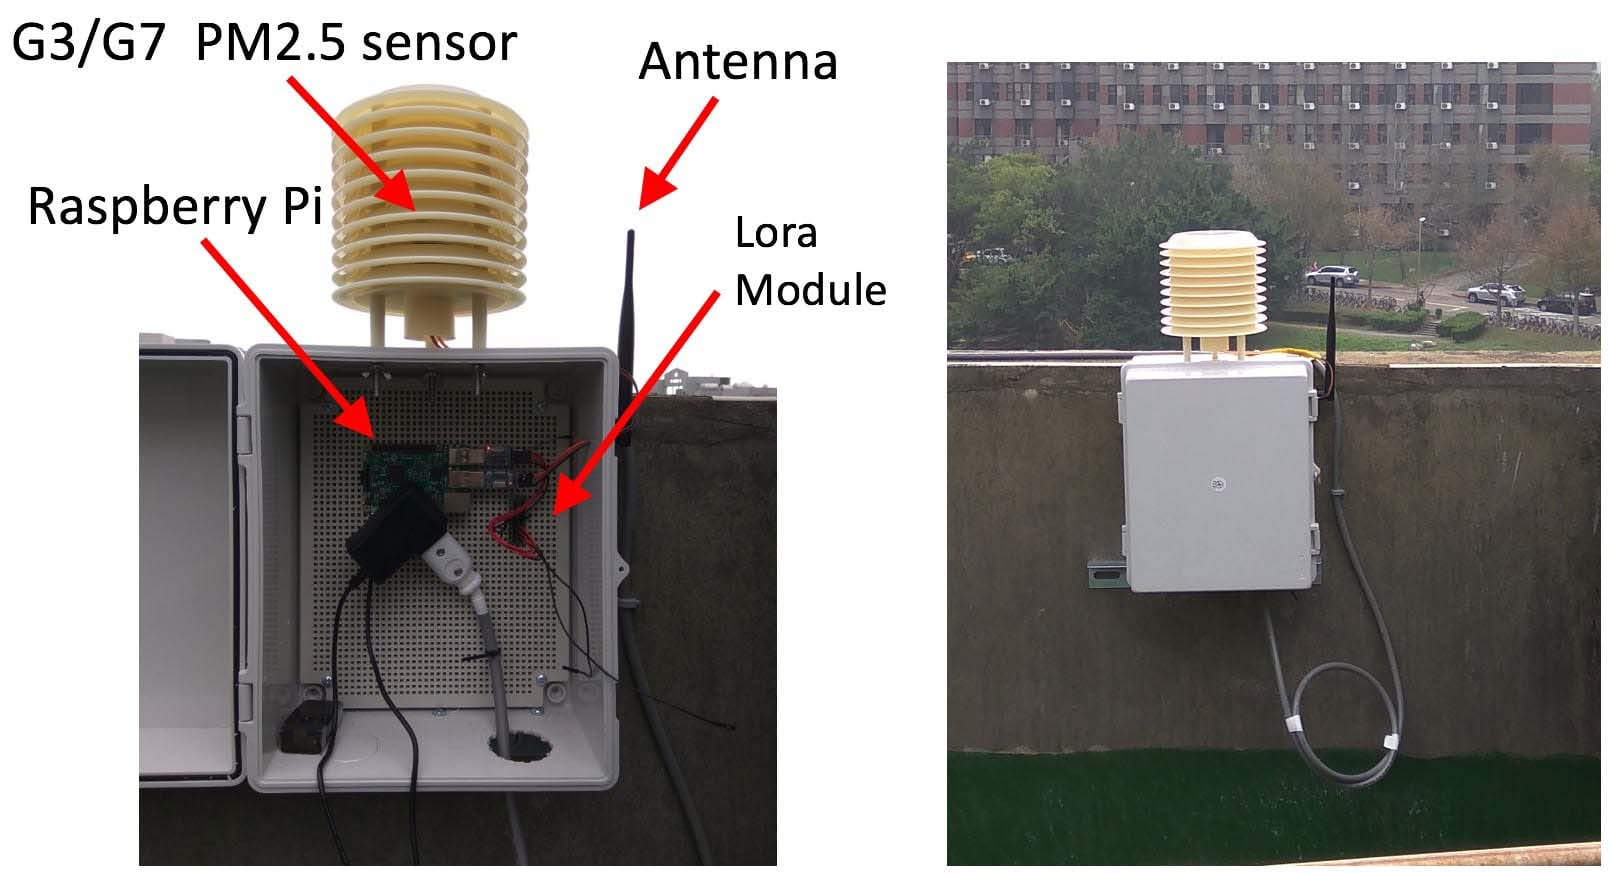
\includegraphics[width=.9\textwidth]{resources/smart-campus-example.png}\\
      \footnotesize{Retirado do artigo disponível em https://ieeexplore.ieee.org/abstract/document/8288154}
    \end{figure}
  \end{frame}

  \begin{frame}{Introdução}
    \framesubtitle{Aplicação - Smart Campus}
    \begin{figure}[ht]
      \centering
      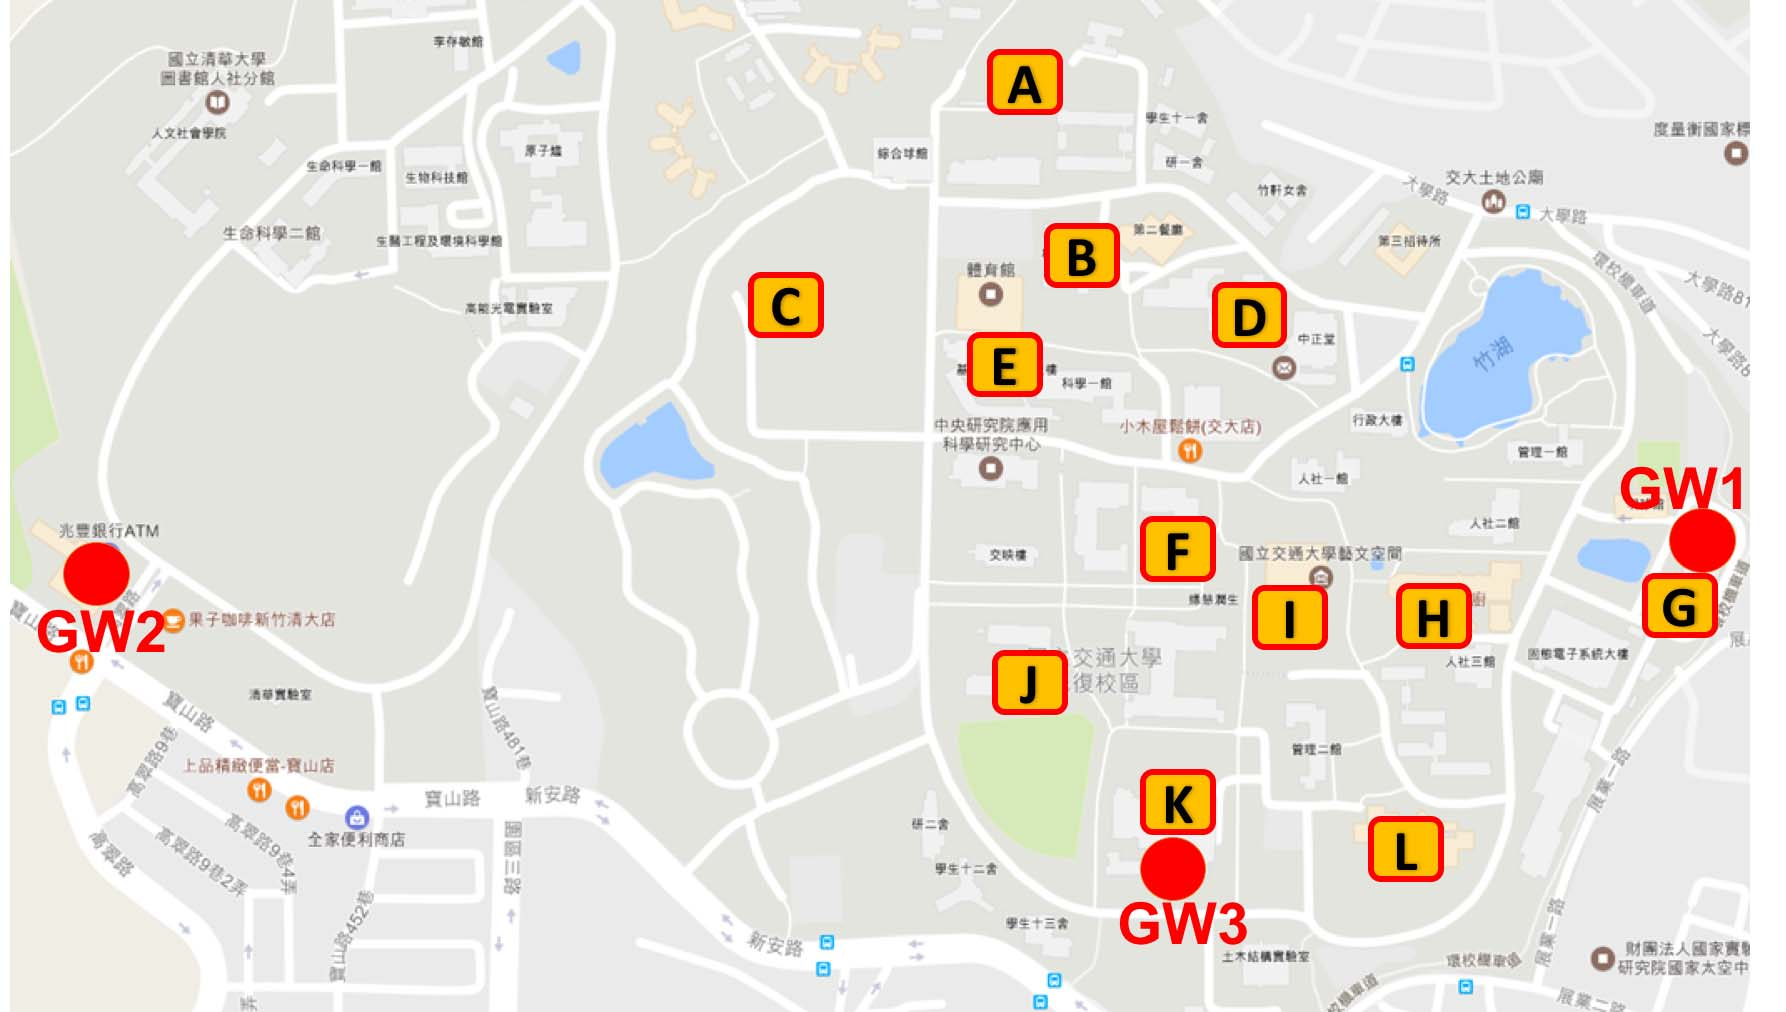
\includegraphics[width=.9\textwidth]{resources/smart-campus-locations.png}\\
      \footnotesize{Retirado do artigo disponível em https://ieeexplore.ieee.org/abstract/document/8288154}
    \end{figure}
  \end{frame}

  \begin{frame}{Introdução}
    \framesubtitle{Redes de Sensores Sem Fio}
    \begin{figure}[ht]
      \centering
      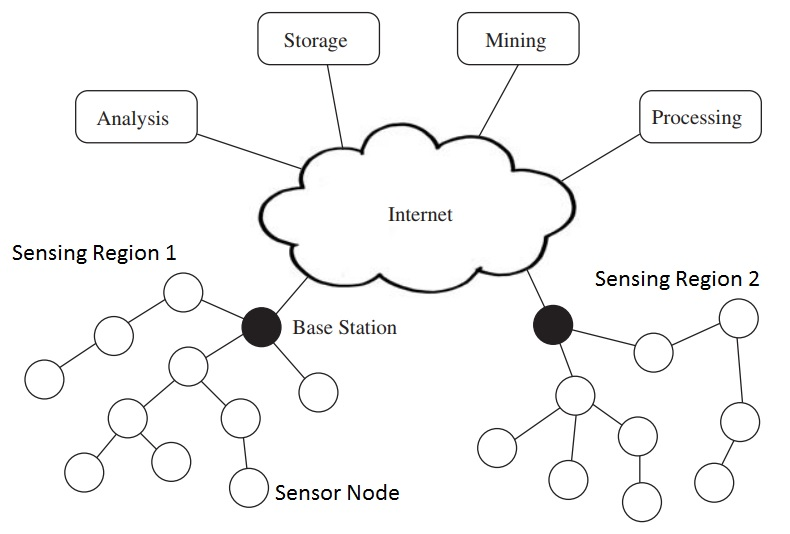
\includegraphics[width=.8\textwidth]{resources/Wireless-Sensor-Networks-WSN.jpg}\\
      \footnotesize{Retirado do site https://getelectronicandmobilenews.blogspot.com/2019/03/basics-of-wireless-sensor-networks-wsn.html}
    \end{figure}
  \end{frame}


  \begin{frame}{Introdução}
    \framesubtitle{Propagação por Multiplos Caminhos}
    \begin{figure}[ht]
      \centering
      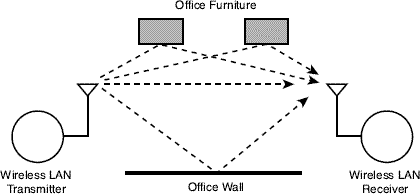
\includegraphics[width=\textwidth]{resources/multipath.png}\\
      \footnotesize{Retirado do site https://sourcedaddy.com/networking/multipath-propagation.html}
    \end{figure}
  \end{frame}

  \begin{frame}{Introdução}
    \framesubtitle{Interferência}
    \begin{itemize}
      \item \alert{Interferência Externa}             \\ Ocorre quando transmissores externos utilizam a mesma faixa de frequência
      \item \alert{Interferência Co-canal}            \\ Ocorre em sistemas com múltiplos usuários que utilizam o mesmo canal
      \item \alert{Interferência de Canal Adjacente}  \\ Ocorre quando uma transmissão é realizada muito proxima de um receptor que está recebendo transmissões de um outro transmissor
    \end{itemize}
  \end{frame}

  \begin{frame}{Introdução}
    \framesubtitle{Padrões e Tecnologias de Redes Sem Fio}
    \begin{figure}[ht]
      \centering
      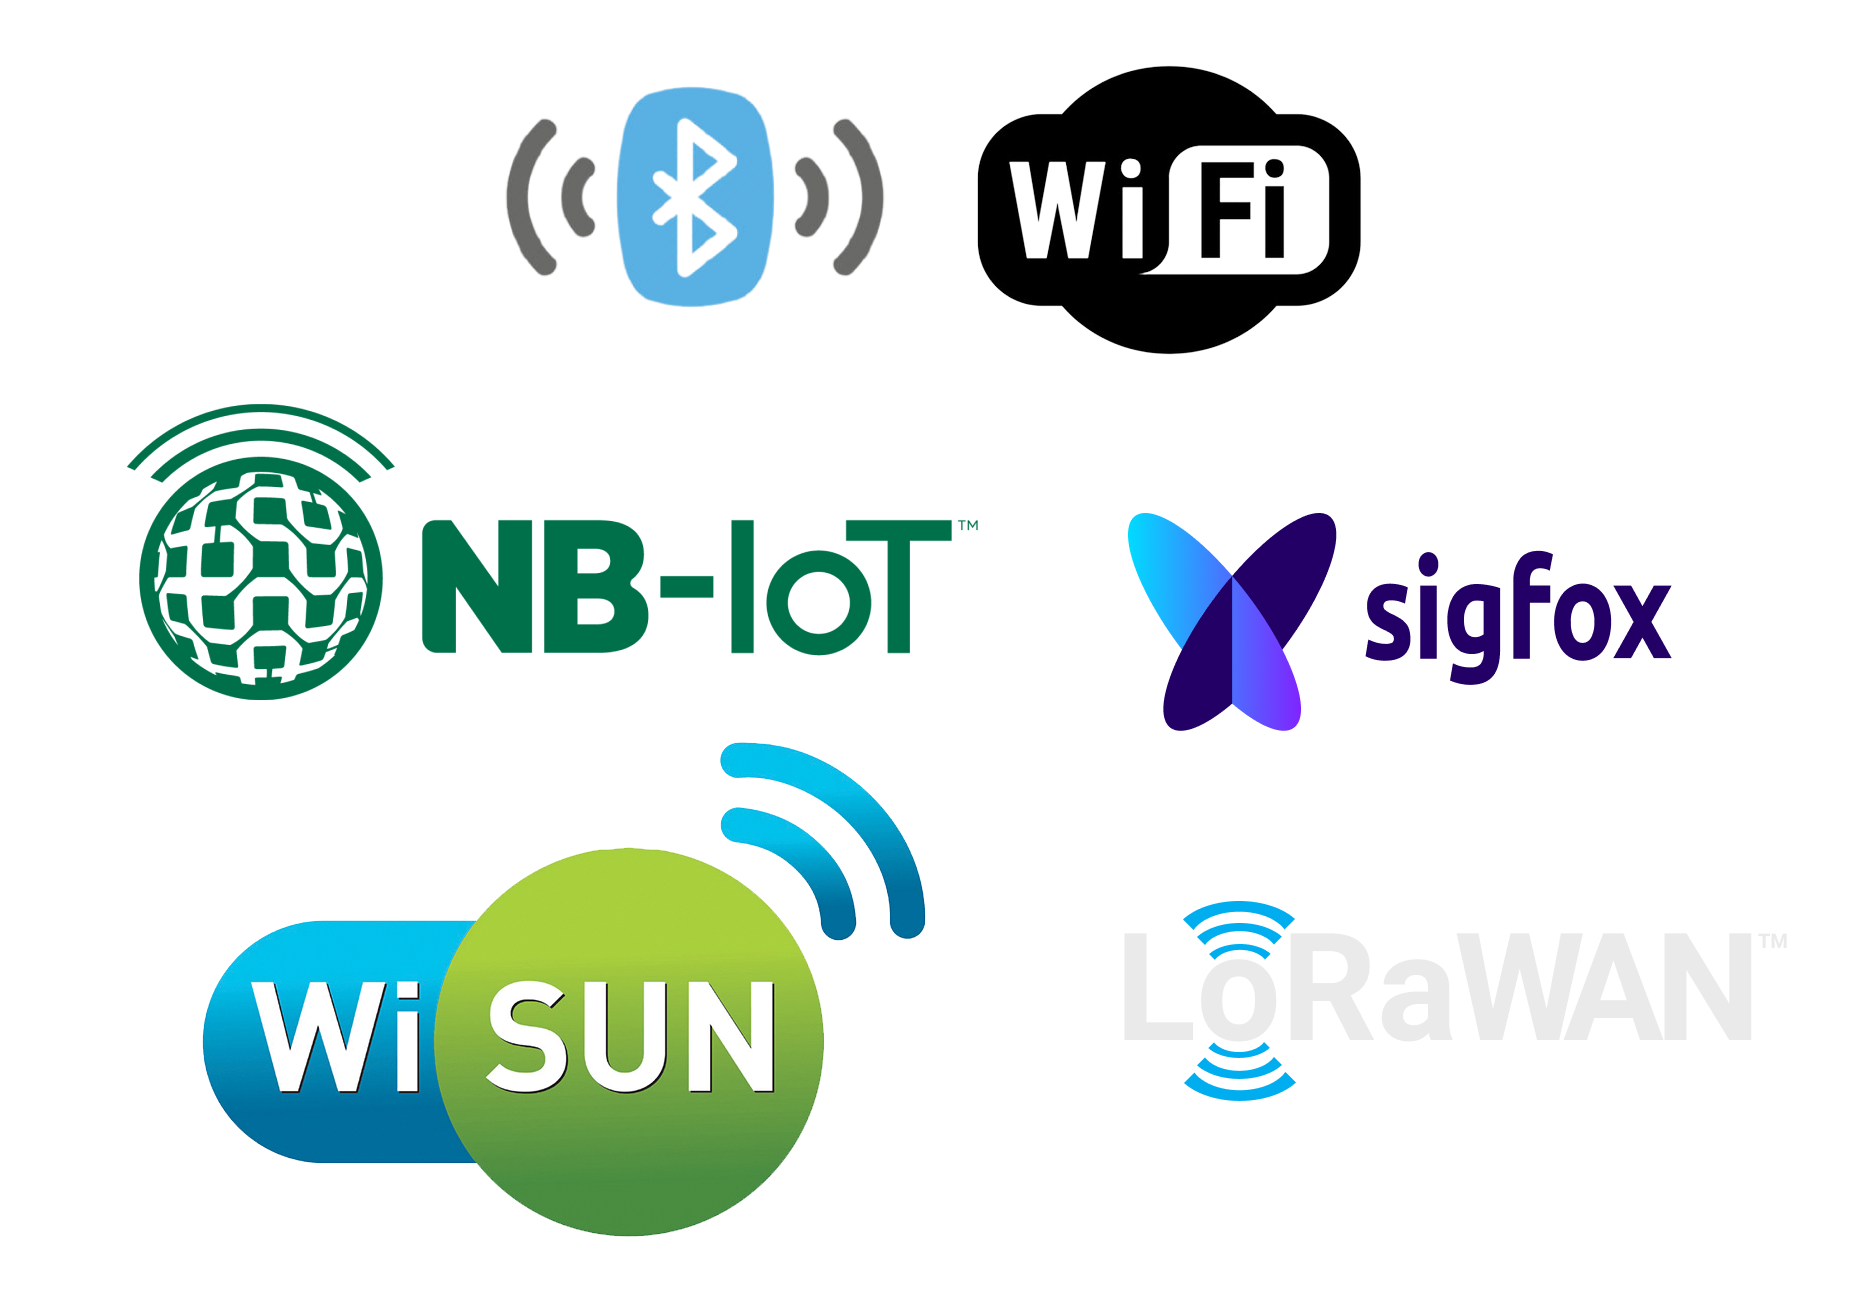
\includegraphics[width=0.8\textwidth]{resources/tecnologias-sem-fio.png}\\
      \footnotesize{Montagem criada pelo autor a partir das logos originais}
    \end{figure}
  \end{frame}

  \begin{frame}{Introdução}
    \framesubtitle{Justificativa e Relevância do Trabalho}
    \begin{figure}[ht]
      \centering
      Artigo \emph{A dataset to evaluate ieee 802.15.4g sun for dependable low-power wireless communications in industrial scenarios}
      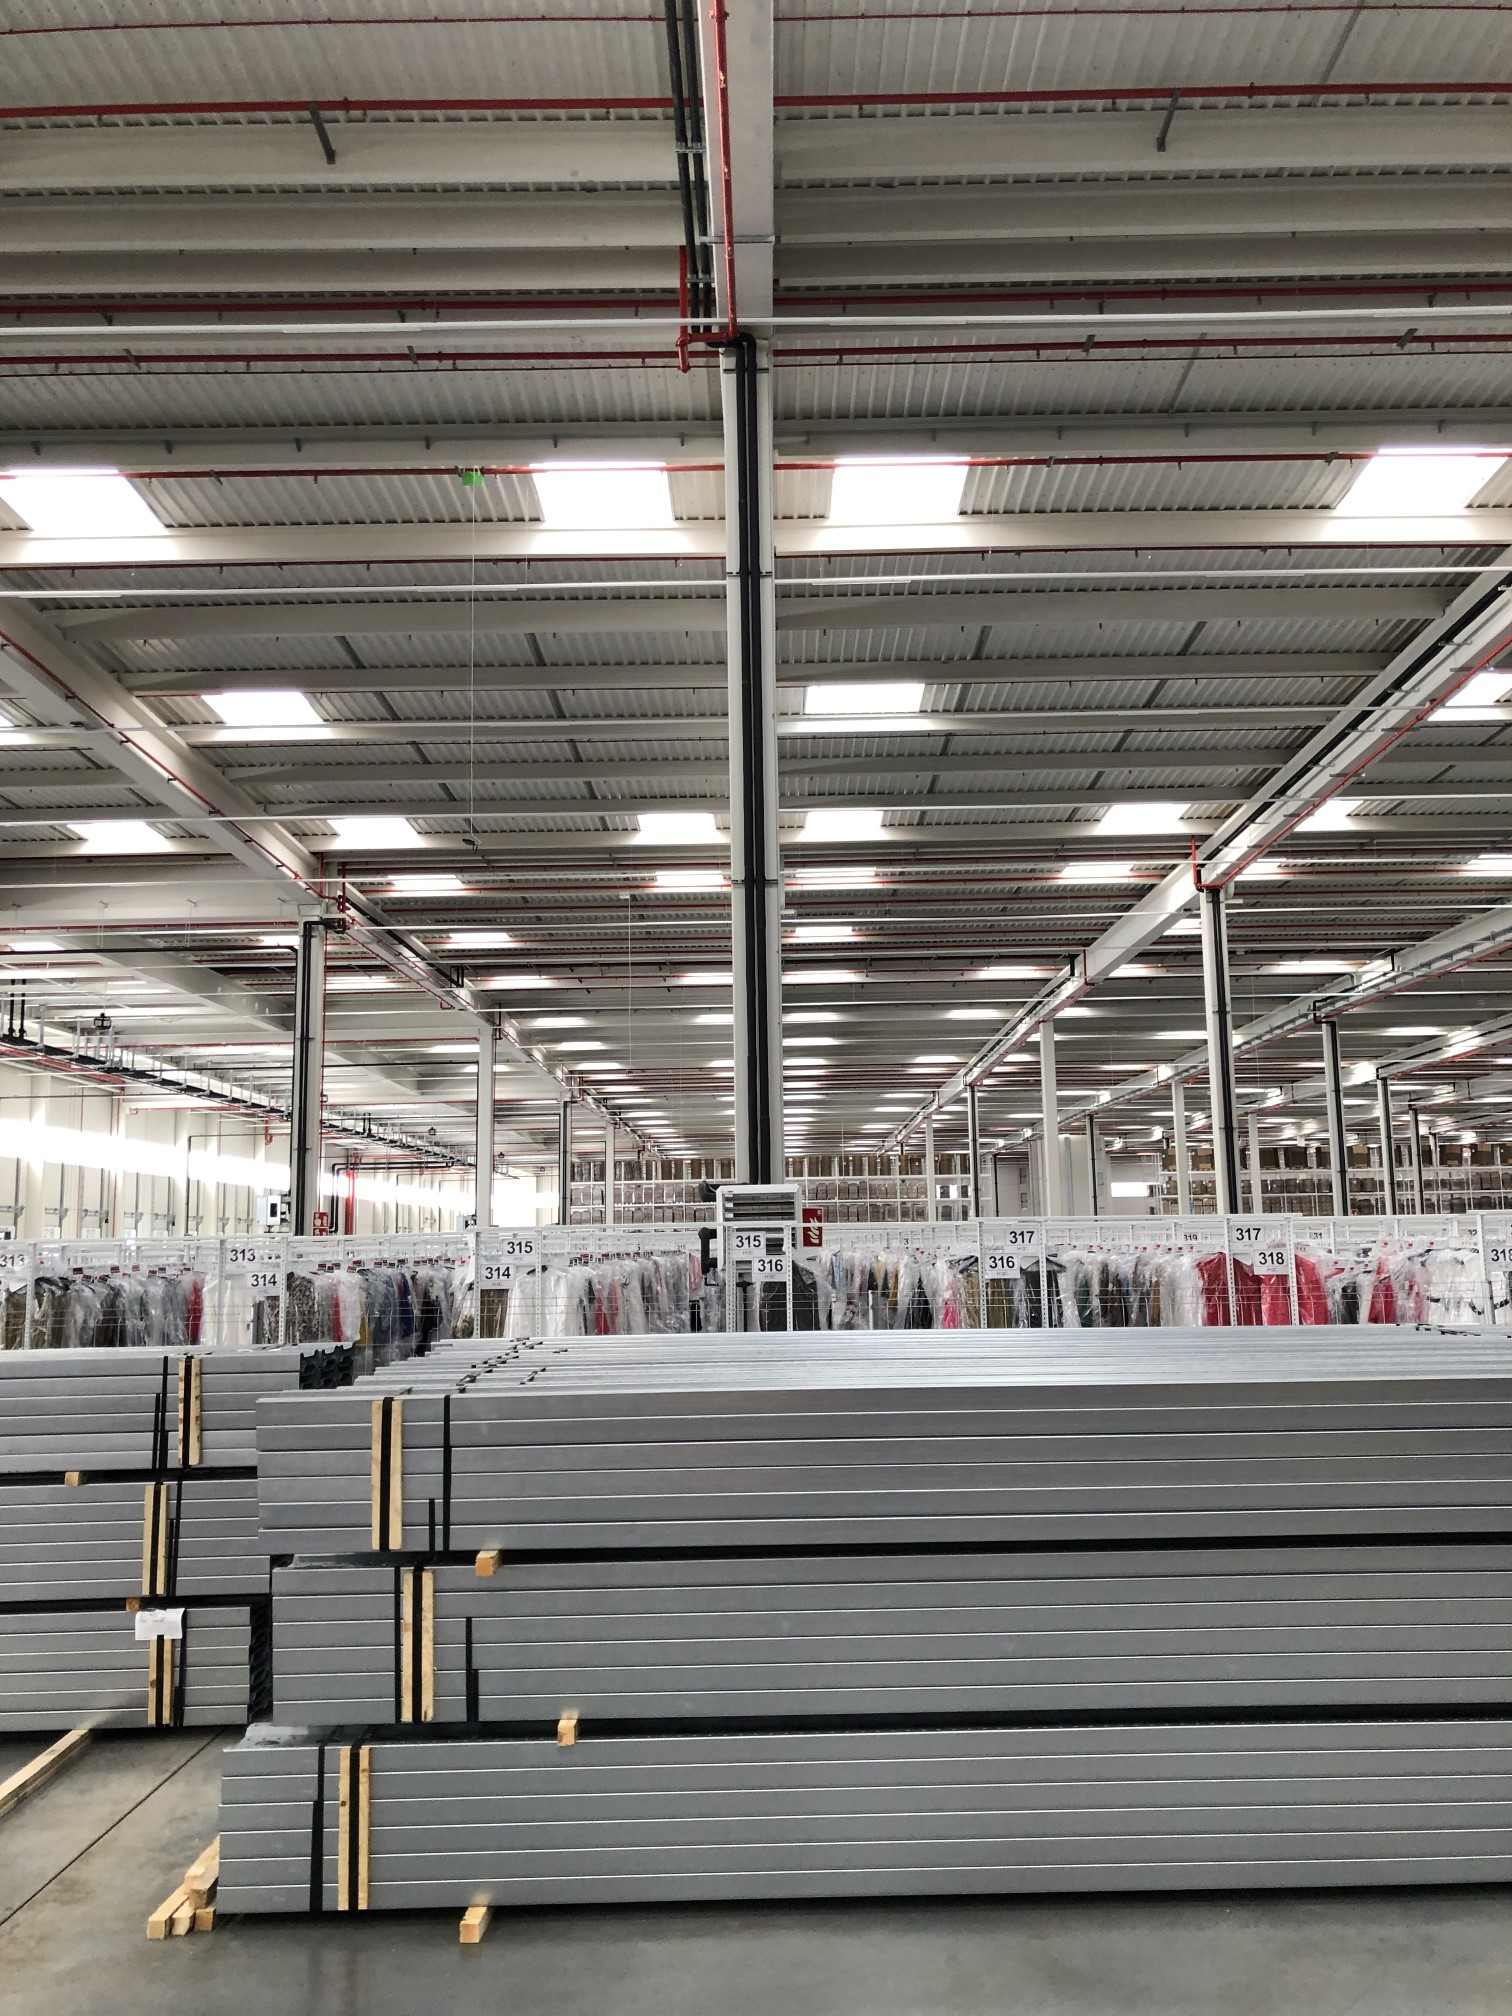
\includegraphics[width=0.3\textwidth]{resources/smart-industrie-example.png}
      \includegraphics[width=0.3\textwidth]{resources/smart-industrie-example2.png}
      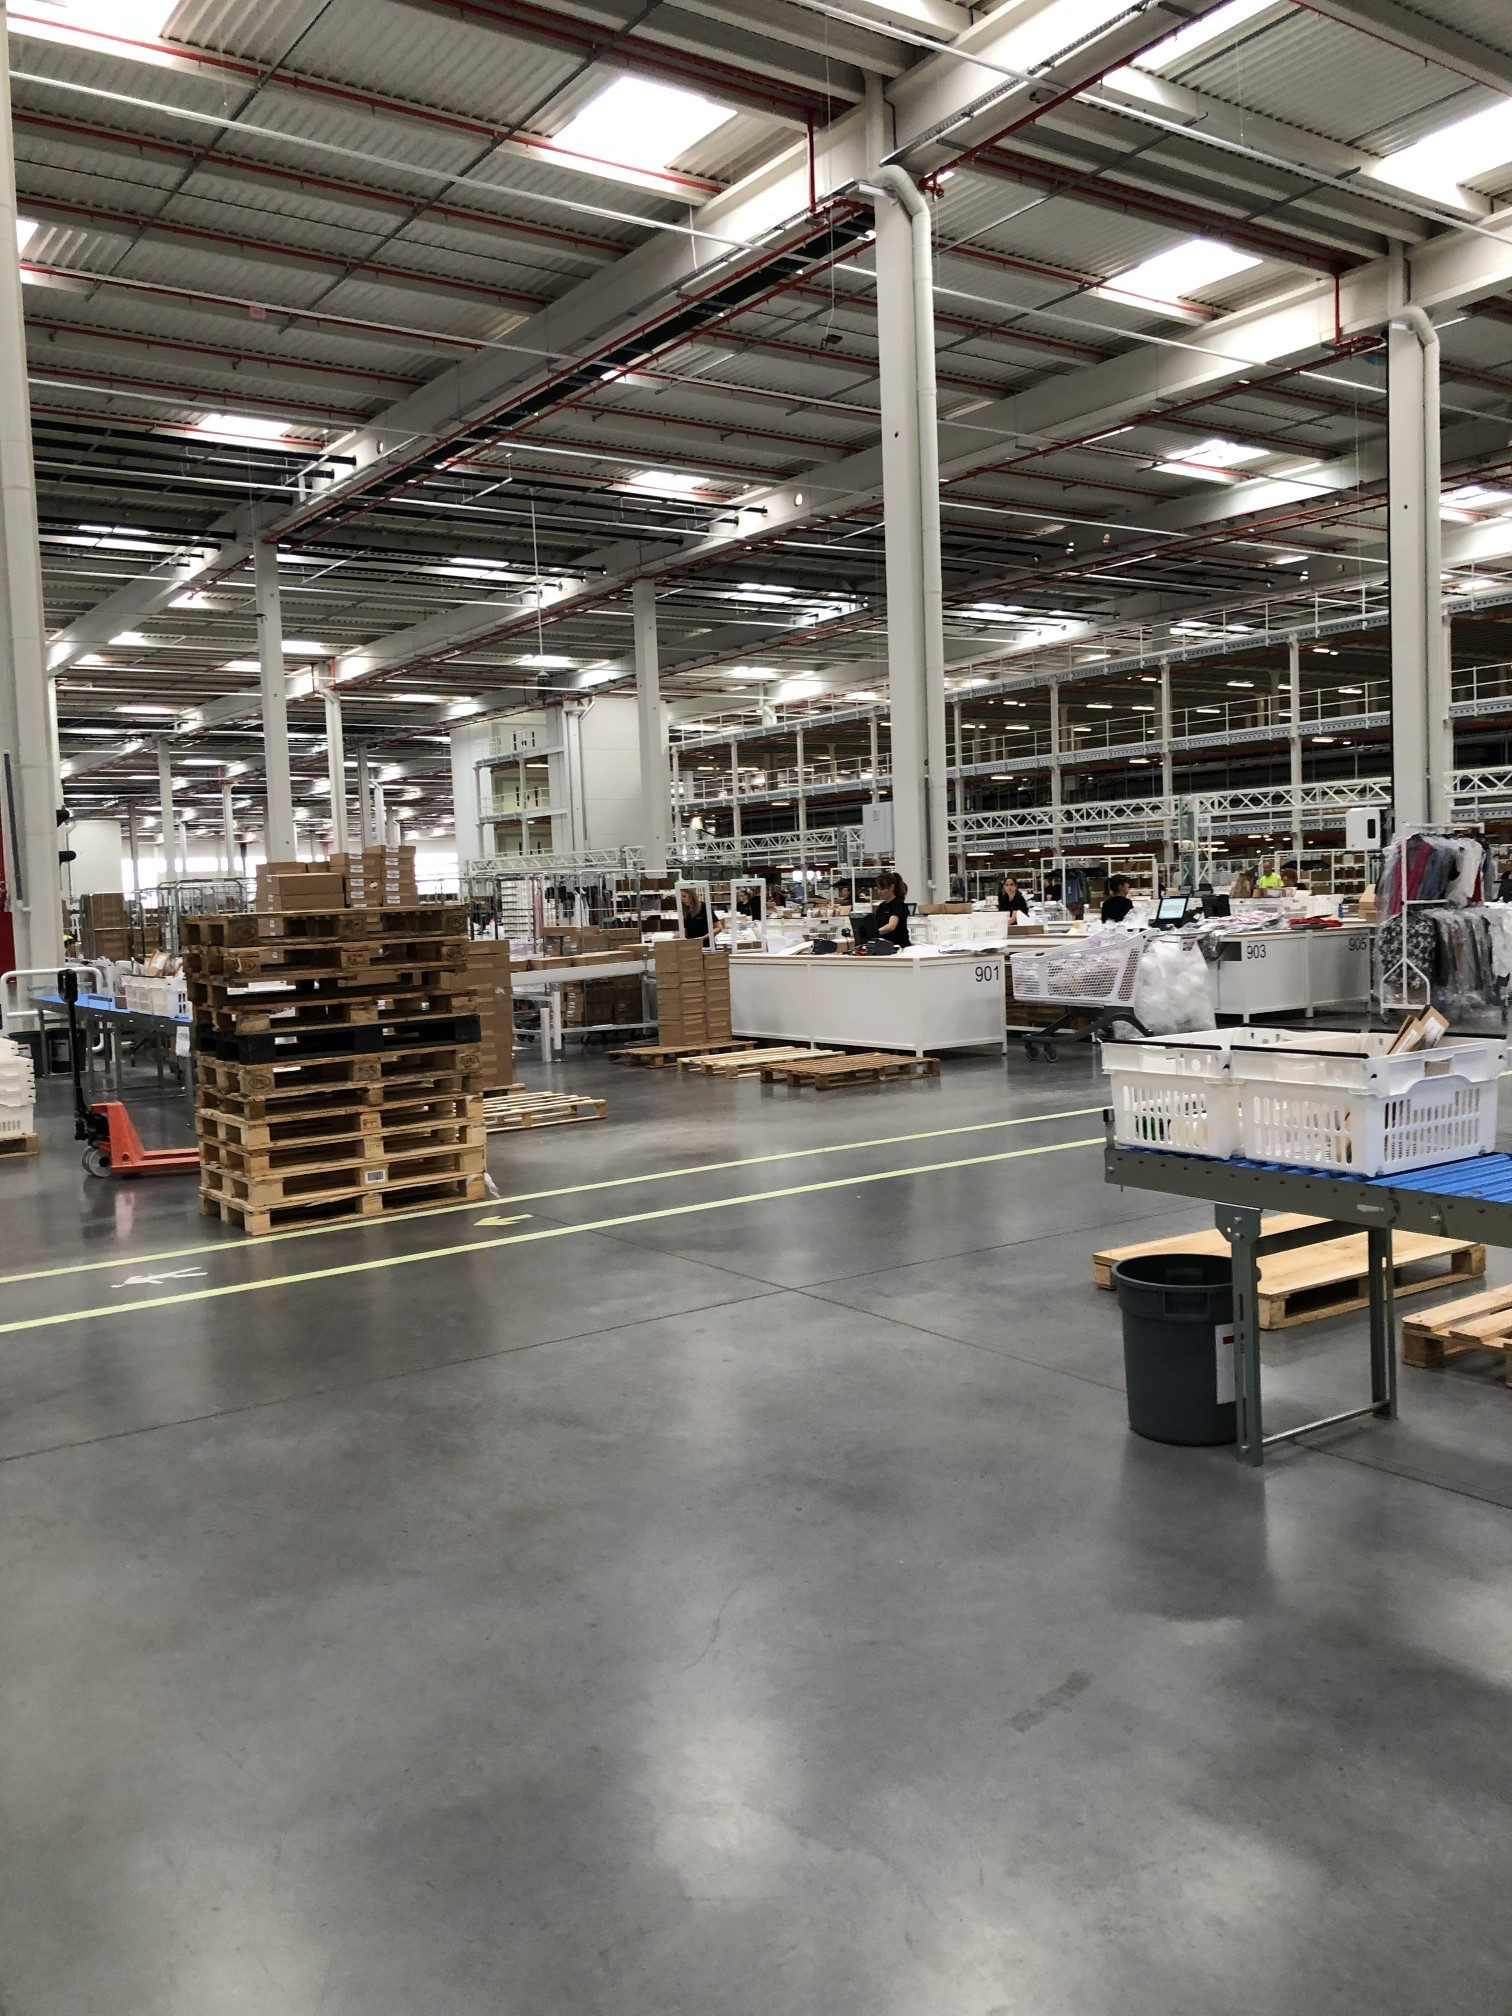
\includegraphics[width=0.3\textwidth]{resources/smart-industrie-example3.png}\\
      \footnotesize{Retirado do artigo disponível em https://www.mdpi.com/2306-5729/5/3/64}
    \end{figure}
  \end{frame}

  \begin{frame}{Introdução}
    \framesubtitle{Justificativa e Relevância do Trabalho}
    Coletar os dados de uma RSSF e analisar o desempenho as modulações \alert{SUN-FSK}, \alert{SUN-OQPSK} e \alert{SUN-OFDM}, definidas no padrão \alert{IEEE 802.15.4g SUN} no ambiente Smart Building

    \vskip .5cm

    \begin{block}{Desafios do cenário}
      \begin{itemize}
        \item Propagação por múltiplos caminhos
        \item Falta de linha de visada
      \end{itemize}
    \end{block}
  \end{frame}


  \begin{frame}
    \usebeamerfont{title}%
    \usebeamercolor[fg]{title}%
    \vskip 0.5cm
    \raggedright Obrigado!
    \vskip-.5\baselineskip
    \begin{pgfpicture}
      \pgfsetlinewidth{2pt}
      \pgfsetroundcap
      \pgfsetdash{{0pt}{4pt}}{0cm}

      \pgfpathmoveto{\pgfpoint{0mm}{0mm}}
      \pgfpathlineto{\pgfpoint{\textwidth}{0mm}}

      \pgfusepath{stroke}
    \end{pgfpicture}

    % Input the subtitle
    \usebeamerfont{subtitle}%
    \usebeamercolor[fg]{subtitle}%
    \begin{minipage}{\textwidth}
      \raggedright%
      Felipe Ferreira Bezerra da Silva%
    \end{minipage}\vskip.25\baselineskip

    % Input the author's name
    \usebeamerfont{author}%
    \usebeamercolor[fg]{author}%

    \raggedright%
    felipeffbs3x@gmail.com
    \vskip 1cm

    \begin{figure}[b]
      
\includegraphics[width=.25\textwidth]{./fibeamer/logo/zut/ifpb.png}
      \hspace{1cm}
      
\includegraphics[width=.25\textwidth]{./fibeamer/logo/zut/gcompi.png}
    \end{figure}
  \end{frame}


\end{darkframes}
\end{document}
